%%%%%%%%%%%%%%%%%%%%%%%%%%%%%%%%%%%%%%%%%
% Towards a portable solar/wind replacement for gas generators
%
% The document layout is based on the Arsclassica Article v1.1 template from:
% http://www.LaTeXTemplates.com
%
% Original author:
% Lorenzo Pantieri (http://www.lorenzopantieri.net) with extensive modifications by:
% Vel (vel@latextemplates.com)
%
% License:
% CC BY-NC-SA 3.0 (http://creativecommons.org/licenses/by-nc-sa/3.0/)
%
%%%%%%%%%%%%%%%%%%%%%%%%%%%%%%%%%%%%%%%%%

%----------------------------------------------------------------------------------------
%	PACKAGES AND OTHER DOCUMENT CONFIGURATIONS
%----------------------------------------------------------------------------------------

\documentclass[
10pt, % Main document font size
letterpaper, % Paper type, use 'letterpaper' for US Letter paper
oneside, % One page layout (no page indentation)
%twoside, % Two page layout (page indentation for binding and different headers)
headinclude,footinclude, % Extra spacing for the header and footer
BCOR5mm, % Binding correction
]{scrartcl}

\input{structure.tex} % Include the structure.tex file which specified the document structure and layout

\hyphenation{Fortran hy-phen-ation} % Specify custom hyphenation points in words with dashes where you would like hyphenation to occur, or alternatively, don't put any dashes in a word to stop hyphenation altogether

\usepackage{tikz}
\usetikzlibrary{plotmarks}

% GNUPLOT required
\usepackage{verbatim}
\usepackage{float}


%----------------------------------------------------------------------------------------
%	TITLE AND AUTHOR(S)
%----------------------------------------------------------------------------------------

\title{\normalfont\spacedallcaps{Towards a portable solar/wind replacement for gas generators}} % The article title

\subtitle{as far as we can get for now}

\author{\spacedlowsmallcaps{Jillian Ada Burrows\textsuperscript{1}}} % The article author(s) - author affiliations need to be specified in the AUTHOR AFFILIATIONS block

\date{} % An optional date to appear under the author(s)

%----------------------------------------------------------------------------------------

\begin{document}

%----------------------------------------------------------------------------------------
%	HEADERS
%----------------------------------------------------------------------------------------

\renewcommand{\sectionmark}[1]{\markright{\spacedlowsmallcaps{#1}}} % The header for all pages (oneside) or for even pages (twoside)
%\renewcommand{\subsectionmark}[1]{\markright{\thesubsection~#1}} % Uncomment when using the twoside option - this modifies the header on odd pages
\lehead{\mbox{\llap{\small\thepage\kern1em\color{halfgray} \vline}\color{halfgray}\hspace{0.5em}\rightmark\hfil}} % The header style

\pagestyle{scrheadings} % Enable the headers specified in this block


%----------------------------------------------------------------------------------------
%	TITLE
%----------------------------------------------------------------------------------------

\maketitle % Print the title/author/date block

%----------------------------------------------------------------------------------------
%	ABSTRACT
%----------------------------------------------------------------------------------------

\section*{Abstract} % This section will not appear in the table of contents due to the star (\section*)
\paragraph{TBD}

%----------------------------------------------------------------------------------------
%	AUTHOR AFFILIATIONS
%----------------------------------------------------------------------------------------

\let\thefootnote\relax\footnotetext{\textsuperscript{1} \textit{Geeks Without Bounds, Colfax, Oregon, USA}}

%----------------------------------------------------------------------------------------
%	TABLE OF CONTENTS & LISTS OF FIGURES AND TABLES
%----------------------------------------------------------------------------------------

\setcounter{tocdepth}{3} % Set the depth of the table of contents to show sections and subsections only

\tableofcontents % Print the table of contents

\listoffigures % Print the list of figures

\listoftables % Print the list of tables


%----------------------------------------------------------------------------------------

\newpage % Start the article content on the second page, remove this if you have a longer abstract that goes onto the second page

%----------------------------------------------------------------------------------------
%	INTRODUCTION
%----------------------------------------------------------------------------------------

\section{Goal}

Create a semi portable unit comparable in size and power output to a standard gasoline or propane based electrical generator found in a typical hardware store. These typically provide anywhere from 1000 to 7500 W in power output and last for about 8 hours running with a full tank at half the rated wattage. These are commonly used without knowing how much power one actually needs. Because it provides more than enough power for a given situation, it lasts a little longer than the half power rating. We can either take the approach of creating a system which is equivalent to a generator working at half power, or we can take the approach that all the power is not needed and most of the energy contained in the gasoline is wasted while the engine runs creating noise pollution anywhere from 56dB to 78+dB.

\subsection{Common Generator Models}

In order to gain a better understanding of what is available on the market, the author started browsing the internet for common generators available at Walmart, Home Depot, Lowe's, and other similar outlets. A wide range of power outputs were found. The results are summarized below.

\begin{table}[hbt]
\caption{Table of Generators}
\centering
\begin{tabular}{cccccc}
\toprule

\multicolumn{4}{l}{\textbf{Generator Name}} \\
\textbf{Surge W} & \textbf{Running W} & \textbf{Weight} & \textbf{Tank Size} & \textbf{Sound Level} & \textbf{Watt Hour rate} \\

\midrule
\multicolumn{4}{l}{Sportsman 1000W Inverter Generator} \\
1000W & 800W & 52lbs & 0.55G & 56+dB & 6.3h at 400W \\

\midrule
\multicolumn{4}{l}{Honda 2000W Inverter Generator} \\
2000W & 1600W & 45.6lbs & 0.95G & 59+dB & 6h at 800W \\

\midrule
\multicolumn{4}{l}{Sportsman 2000W Generator} \\
2000W & 1400W & 53lbs & 1.2G & 65+dB & 9h at 700W \\

\midrule
\multicolumn{4}{l}{Honda 5000W Generator} \\
5000W & 4500W & 173lbs & 6.3G & 73+dB & 11h at 2250W \\

\midrule
\multicolumn{4}{l}{Ryobi 5500W Generator} \\
6875W & 5500W & 194lbs & 6G & 78+dB & 9h at 2750W \\

\midrule
\multicolumn{4}{l}{Dewalt 7000W Generator} \\
8750W & 7000W & 192lbs & 7.5G & ?dB & 11h at 4500W \\

\bottomrule
\end{tabular}
\label{tab:generators}
\end{table}

\subsection{Summary of Generators}
\begin{enumerate}[noitemsep]
\item Each produces a lot of noise.
\item Each weighs anywhere from 46lbs to 192lbs.
\item Cost anywhere from [\$1.30 @ \$2.38/G, \$1.71 @ \$3.117/G] to [\$17.85 @ \$2.38/G, \$23.37 @ \$3.117/G] with one tank of gas.
\item Produces anywhere from 2520Wh to 49500Wh with one tank.
\item It cost anywhere from \$4.95/24h to \$6.51/24h to run the smallest model (9600Wh/day) and anywhere from \$38.95/24hr to \$50.99/24hr to run the largest model (108000Wh/day).
\end{enumerate}

%------------------------------------------------

\section{Typical Power Requirements}

Gasoline generators are capable of putting out a decent amount of power, but they don't always regulate their gas usage much while not under load. A lot of the newer ones try to be more efficient, but there's still a decent amount of waste of energy at low loads. Also, gasoline generators have been around since the age of electricity hogging devices like CRTs -- now replaced by highly energy efficient LED flat panel displays. Not many people use as much power from a generator as the generator can provide.

\subsection{Power Requirements for Typical Devices}

In order charge a modern phone, it takes a minimum of 1.5A @ 5V or 7.5W. A tablet (or more recently, phones) takes at least 2.1A @ 5V or 10.5W. A Samsung Galaxy S7 Edge takes 1.8A @ 9V or 16.2W for 1:39. A Chromebook I have laying around takes 2A @ 12V or 24W and about an hour to charge. The laptop I typing on takes 3.42A @ 19V or approximately 65 W and about two hours to charge. The new modern USB-C spec has a charging mode which can negotiate up to 5A @ 20V or 100W. Standard lamps with LED or CFL lighting can be run at 15W to 20W. An LED TV can take anywhere from 24.2W (Vizio E1-A1 24") to 147W (Samsung 6 Series UE40JU6400K 4K UltraHD 40"). A regular sized refrigerator/freezer combo unit takes 70W to keep it running (I'm sure there's some variance in that so it probably spikes intermittently).

In many situations, people will have medical equipment which needs to be powered. Nebulizer machines can take anywhere from around 50W to 204W. A CPAP machine seems to fall within the same range (I'm having trouble finding the exact specs online for any model). A Fresenius 2008K@home dialysis machine uses 12.5A @ 120V or 1500W for as long as it takes to cycle all your blood through the system.

\begin{table}[hbt]
\caption{Table of Common Devices}
\centering
\begin{tabular}{lccccc}

\toprule
\textbf{Device} & \textbf{W} & \textbf{A} & \textbf{V} & \textbf{T} & \textbf{Wh} \\

\midrule
Generic Cellphone & 7.5W & 1.5A & 5V & 6h & 45Wh \\
Generic 3.0A USB Charger & 15W & 3A & 5V & 3h & 45Wh \\
Generic Tablet & 10.5W & 2.1A & 5V & 6h & 63Wh \\
Samsung Galaxy S7 Edge* & 16.2W & 1.8A & 9V & 1h 39m & 26.73Wh \\
ASUS C100P Chromebook* & 24W & 2A & 12V & 2h & 48Wh \\
ASUS Q522U Notebook PC* & 65W & 3.42A & 19V & 2h & 130Wh \\
LED or CFL Lamp* & 20W & $\frac{1}{6}$A & 120V & 8h & 160Wh \\
Vizio 24" 1080 HDTV* & 24.2W & ? & 120V & 4h & 96.8Wh \\
Samsung 4K UltraHD 40"* & 147W & ? & 120V & 4h & 588Wh \\
Refrigerator/Freezer* & 70W+40W & ? & 120V & 24h & 1680Wh \\
\midrule
Nebulizer* & 50W & 0.42A & 120V & 1h & 50Wh \\
CPAP* & 50W & 0.42A & 120V & 8h & 400Wh \\
Dialysis* & 1500A & 12.5A & 120V & \textit{varies} & \textit{varies} \\

\bottomrule
\end{tabular}
\label{tab:devices}
\end{table}
\paragraph{*}Uses an external AC adapter to charge.

\subsection{Phone}

Let's go really basic for a moment. Let's assume all we want for emergency situations is our phone and a lamp. We can go for the lowest common denominator and just provide a USB port for charging that provides 2.1A and requires up to 8 hours to charge newer phones. That's 16.8Ah/per phone charge and since this is an emergency situation it would be nice to charge it at least three times. That brings us to 50.4Ah or 252Wh with a 2.1A discharge rate.

\subsection{Phone and Lamp}




\subsection{Phone, Tablet, and Lamp}


\subsection{Phone, Tablet, Laptop, and Lamp}


%------------------------------------------------

\section{Choosing a Battery}

In order to choose the proper battery we need to know the number of Amp-Hours [Ah] we need to produce a certain number of Watt-Hours [Wh] in AC. This means we need to know the conversion efficiency of our inverter, since one hasn't been chosen, we will assume a typical conversion rate of 90\%.

\begin{equation}
Necessary_{Wh} = \frac{AC_{Wh}}{Conversion_{Efficiency}}
\label{eq:1}
\end{equation}

\begin{equation}
Necessary_{Ah} = \frac{AC_{Wh}}{Conversion_{Efficiency} \cdot Battery_{Vdc}}
\label{eq:2}
\end{equation}

\subsection{Battery Types}
Additionally, we need to take into consideration what kind of battery we're using. We can choose from:
\begin{itemize}[noitemsep]
\item Lead-acid
	\begin{itemize}
	\item Flooded Cell
	\item AGM
	\item Gelled Electrolyte
	\end{itemize}
\item Nickel-Cadmium (NiCad)
\item Nickel-Metal Hydride (NiMH) 
\item Lithium-ion (Li-ion)
\item Lithium-polymer (LiPo)
\end{itemize}

Each type of battery has it's own kind of characteristics. These can encompass how much charge the battery can hold, how well the battery performs at a certain temperature, how long it lasts while powering a load, the ability to hold a charge in storage, how quickly it can be charged, and a number of other parameters. Typically, a solar or wind system will use a lead-acid battery because they are readily available and certain kinds of lead-acid batteries work better in cold weather than others. Lithium-ion batteries are widely used in many devices. Most phones, tablets, and other portable computers use Li-ion because of their energy density. They do have the habit of catching on fire if misused. In the following calculations we'll stick to lead-acid.

\subsection{Battery Discharge Time}
All batteries have a different behavior Lead-acid batteries have a discharge rate which is governed by the rate of the chemical reactions in the acid electrolyte paste. Instead of having a linear relationship as one might expect, there's an exponential relationship governed by Peurkert's Law. The law is typically stated in terms of the Amp-hour rating for a certain period in hours:

\begin{equation}
t = H\left(\frac{C}{I \times H}\right)^k,
\label{eq:3}
\end{equation}

where
\begin{itemize}
\item $t$ is the number of hours until a battery is discharged.
\item $I$ is the current being drawn in Amps.
\item $H$ is the number of hours specified in the N Hour Rate of the battery.
\item $C$ is the capacity in Amp-hours specified for the N Hour Rate of the battery.
\item $k$ is a dimensionless constant called the Peukert Constant (from the name of the law).
\end{itemize}

We can also look at how the actual effective capacity of the battery changes given a specific current draw

\begin{equation}
I_t = C\left(\frac{C}{I \times H}\right)^{k-1},
\label{eq:4}
\end{equation}

where $I_t$ is the effective capacity of the battery and all other variables are the same as above.

\paragraph{34Ah @ 24h rate} The following charts are for a battery with a capacity of 34Ah for a 24h rate:

\begin{figure}[H]
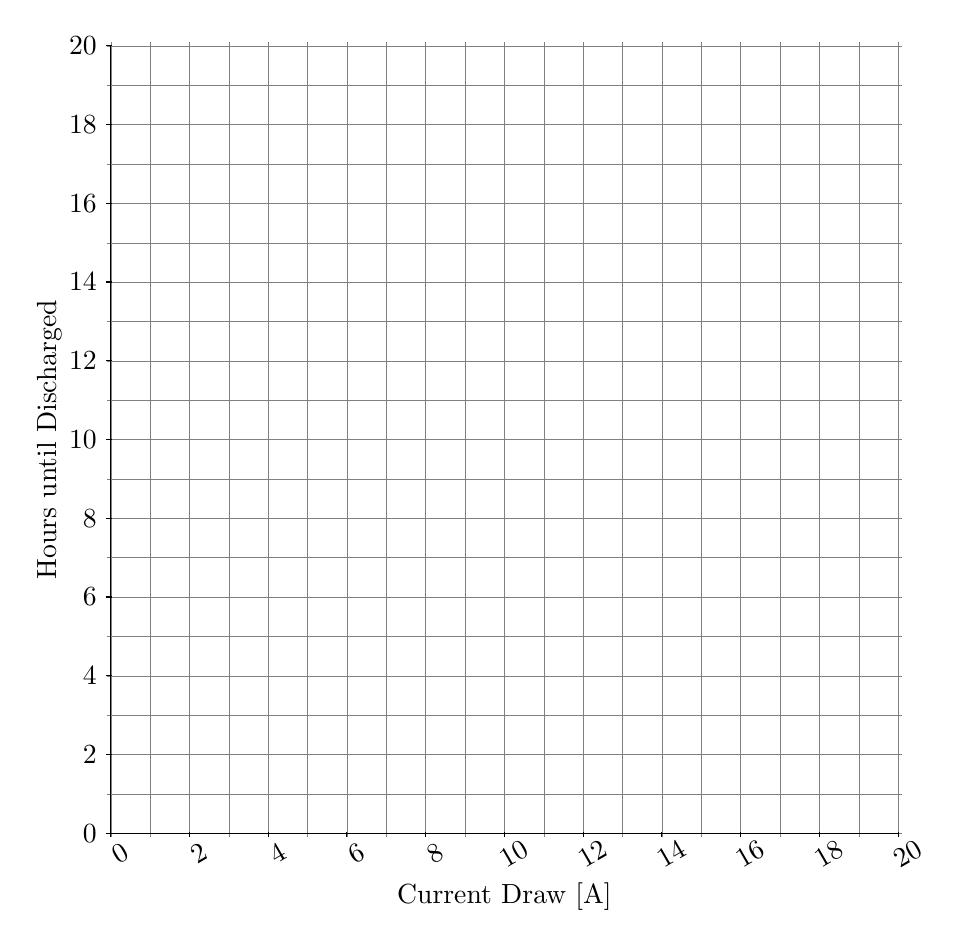
\begin{tikzpicture}[domain=0:20,step=1cm,xscale=0.5,yscale=0.5]

	% Grid
    \draw[ultra thin,color=gray] (-0.1,-0.1) grid (20.1,20.1);

	\draw (0,0) -- coordinate (x axis mid) (20,0);
    	\draw (0,0) -- coordinate (y axis mid) (0,20);

	% Ticks
    	\foreach \x in {0,2,...,20}
     		\draw (\x,1pt) -- (\x,-3pt)
			node[anchor=north,rotate=30] {\x};
    	\foreach \y in {0,2,...,20}
     		\draw (1pt,\y) -- (-3pt,\y) 
     		node[anchor=east] {\y};
     		
    	% Labels      
	\node[below=0.5cm] at (x axis mid) {Current Draw [A]};
	\node[rotate=90, above=0.5cm] at (y axis mid) {Hours until Discharged};
	
	% Plots
    \draw[domain=1.675:20,color=orange] plot[id=x] function{24*((34/(x*24))**1.12)};
    
\end{tikzpicture}
\caption{Time until discharge as a function of current draw on a lead acid battery w/a capacity of 34Ah for a 24h rate.}
\label{fig:TC34Ah}
\end{figure}

\begin{figure}[H]
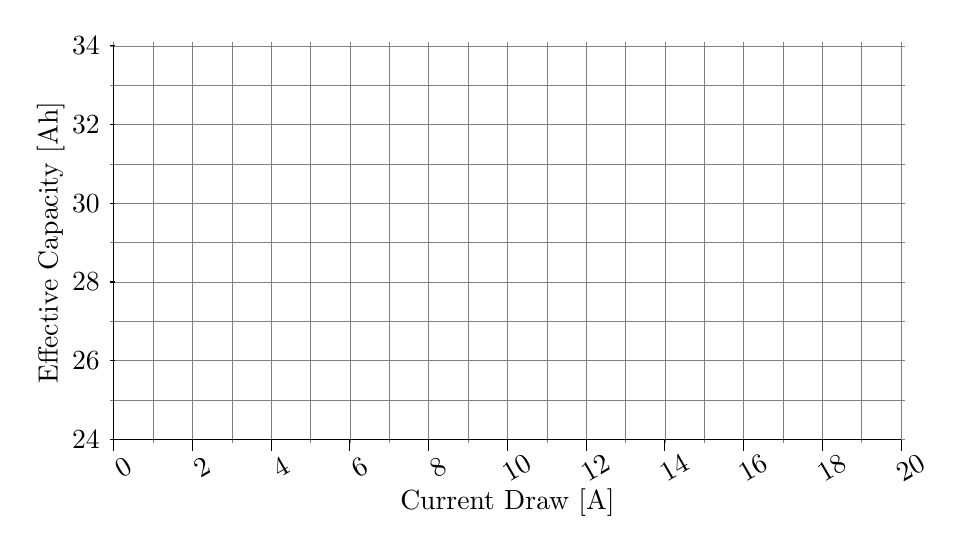
\begin{tikzpicture}[domain=0:20,step=1cm,xscale=0.5,yscale=0.5]

	% Grid
    \draw[very thin,color=gray] (-0.1,23.9) grid (20.1,34.1);

	\draw (0,24) -- coordinate (x axis mid) (20,24);
    	\draw (0,24) -- coordinate (y axis mid) (0,34);

	% Ticks
    	\foreach \x in {0,2,...,20}
     		\draw (\x,24) -- (\x,23.7)
			node[anchor=north,rotate=30] {\x};
    	\foreach \y in {24,26,...,34}
     		\draw (1pt,\y) -- (-3pt,\y) 
     		node[anchor=east] {\y};
     		
    	% Labels      
	\node[below=0.5cm] at (x axis mid) {Current Draw [A]};
	\node[rotate=90, above=0.5cm] at (y axis mid) {Effective Capacity [Ah]};
	
	% Plots
    \draw[domain=1.5:20,color=orange] plot[id=x] function{34*((34/(x*24))**(1.12-1))};
    
\end{tikzpicture}
\caption{Effective capacity as a function of current draw on a lead acid battery w/a capacity of 34Ah for a 24h rate.}
\label{fig:EC34Ah}
\end{figure}

\paragraph{104Ah @ 24h rate} The following charts are for a battery with a capacity of 104Ah for a 24h rate:
\begin{figure}[H]
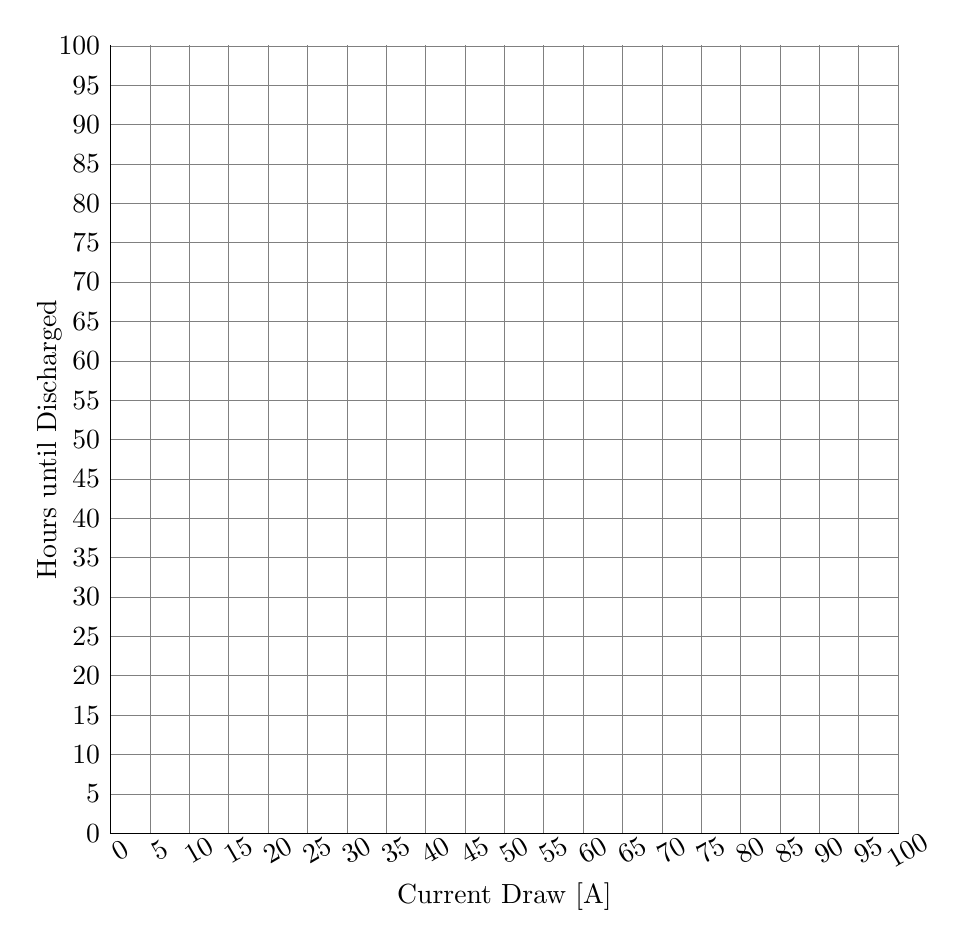
\begin{tikzpicture}[domain=0:100,step=5,xscale=0.1,yscale=0.1]

	% Grid
    \draw[very thin,color=gray] (-0.1,-0.1) grid (100.1,100.1);

	\draw (0,0) -- coordinate (x axis mid) (100,0);
    	\draw (0,0) -- coordinate (y axis mid) (0,100);

	% Ticks
    	\foreach \x in {0,5,...,100}
     		\draw (\x,1pt) -- (\x,-3pt)
			node[anchor=north,rotate=30] {\x};
    	\foreach \y in {0,5,...,100}
     		\draw (1pt,\y) -- (-3pt,\y) 
     		node[anchor=east] {\y};
     		
    	% Labels      
	\node[below=0.5cm] at (x axis mid) {Current Draw [A]};
	\node[rotate=90, above=0.5cm] at (y axis mid) {Hours until Discharged};
	
	% Plots
    \draw[domain=1.3:100,color=red] plot[id=x] function{24*((104/(x*24))**(1.12))};
    
\end{tikzpicture}
\caption{Time until discharge as a function of current draw on a lead acid battery w/a capacity of 104Ah for a 24h rate.}
\label{fig:TC104Ah}
\end{figure}

\begin{figure}[H]
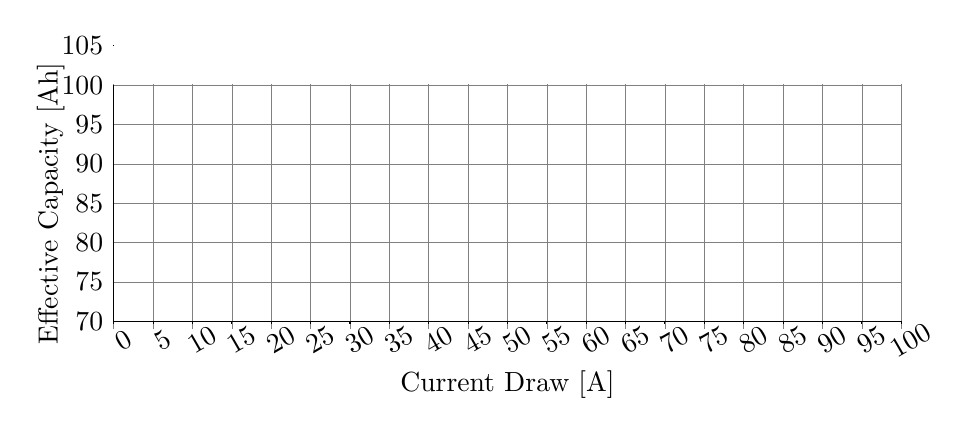
\begin{tikzpicture}[domain=0:100,step=5,xscale=0.1,yscale=0.1]

	% Grid
    \draw[very thin,color=gray] (-0.1,69.1) grid (100.1,100.1);

	\draw (0,70) -- coordinate (x axis mid) (100,70);
    	\draw (0,70) -- coordinate (y axis mid) (0,100);

	% Ticks
    	\foreach \x in {0,5,...,100}
     		\draw (\x,70) -- (\x,69.7)
			node[anchor=north,rotate=30] {\x};
    	\foreach \y in {70,75,...,105}
     		\draw (1pt,\y) -- (-3pt,\y) 
     		node[anchor=east] {\y};
     		
    	% Labels      
	\node[below=0.5cm] at (x axis mid) {Current Draw [A]};
	\node[rotate=90, above=0.5cm] at (y axis mid) {Effective Capacity [Ah]};
	
	% Plots
    \draw[domain=6:100,color=red] plot[id=x] function{104*((104/(x*24))**(1.12-1))};
    
\end{tikzpicture}
\caption{Effective capacity as a function of current draw on a lead acid battery w/a capacity of 104Ah for a 24h rate.}
\label{fig:EC104Ah}
\end{figure}

\subsection{Temperatures Effect on Capacity}

\section{Charging Batteries}



%----------------------------------------------------------------------------------------

\end{document}